% this file is called up by thesis.tex
% content in this file will be fed into the main document

\chapter{Replacement for Graph Community Detection Step} % top level followed by section, subsection
\label{cha:gcn}
% ----------------------- contents from here ------------------------
% 

This chapter presents the replacement created using a Graph
Convolusional Neural Network (GCN) for the \emph{Graph Community Detection
Step} of the Karas pipeline (see \ref{sec:karas-pipeline}). It is
observed that a GCN is able to classify noise and event nodes very
well, even in extremely skewed datasets with less than 10 event nodes.
The chapter begins with an overview of GCNs and how they have been
applied to this problem. The data preparation, visualization and model
evaluation are touched upon next. The chapter concludes with
discussion of the results and next steps.

\section{Primer on Graph Convolusional Neural Networks}
\label{sec:gcn-primer}

\subsection{GNN and graphs}

% TODO mathematical depiction of graphs
GNNs are designed to operate on data which can be represented as
graphs. A graph consists of nodes and edges. Each node may or may not
be connected to one or many nodes, these are referred to as the
neighbors of the node. A graph with all nodes connected to one another
is called a fully connected graph.

An edge may have attributes associated with it, the two most common
attributes being weight and direction. An edge may be directed which
denotes a sense of hierarchy amongst the nodes, or undirected. An edge
may also have a weight to signify a stronger or weaker connection
amongst nodes.

Nodes may also posses attributes associated with themselves, commonly
known as node embeddings. The complexity of the node embedding may
range from a simple scalar quantity to a multi-dimensional tensor,
and depends on the dataset and how the practitioner wishes to sculpt
the graph.

Graphs are primarily classified into two variants.

\begin{enumerate}
\item \textbf{Homogeneous graphs}. Graphs with the same type of nodes
  and edges are referred to as homogeneous graphs. For example, a
  graph representing who follows who on Twitter is a homogeneous
  graph. Here, people are represented as nodes and an edge indicates
  that person A follows person B.
\item \textbf{Heterogeneous graphs}. Graphs with different types of
  nodes and edges are referred to as heterogeneous graphs. For
  example, a graph representing a person's likes and dislikes in
  regards to food items. Here, two entities, namely people and food
  are represented as nodes. The edges also come in two variants ie. a
  'like' and a 'dislike'.
\end{enumerate}
% TODO illustrate types of graphs and their attributes

\subsection{The Message Passing Paradigm}

% TODO illustrate the paradigm
% TODO introduce mathematically?
During each training epoch, a node propagates it's embedding to it's
neighbors and in return receives their embedding. All collected
embeddings are aggregated (for example using a sum, difference or
mean) which becomes the new embedding of the node. This procedure is
done for all nodes of the graph, for each training epoch. The number
of layers in the network determine how far the messages are sent. For
example, for a network with a single layer, each node sends a message
to it's immediate neighbors. With 2 layers, the node also sends a
message to the neighbors of it's immediate neighbors and so forth.

%% \subsection{GNN and it's Variants}

%% GNNs have two primary applications.

%% \begin{enumerate}
%% \item \textbf{Node classification}. This is a semi-supervised learning
%%   setting (although it can also be used in a supervised setting).
%%   Given a graph with nodes associated with a label, the network can be
%%   used to predict the label of unseen nodes.
%% \item \textbf{Graph classification}. In this approach, the network is
%%   trained using several graphs each associated with a label. The
%%   network can then be used to predict the label of an unseen graph.
%% \end{enumerate}


\section{Data Preparation}
\label{sec:gcn-data-prep}

% TODO illustrate data prep procedure
The graphs for the testing and training of the network are constructed
from a combination of the main dataset and a modified version of the
MLP dataset, Figure \ref{fig:gcn-data} illustrates this procedure. A
fully connected graph is constructed, and its node embeddings and node
labels are derived from the main dataset. Thus, each node is thus
assigned a $(x,y,z,t)$ vector as it's node embedding. The node is
assigned a label of 1 if it is an event hit, else a label of 0.

\begin{figure}[h]
  \centering
  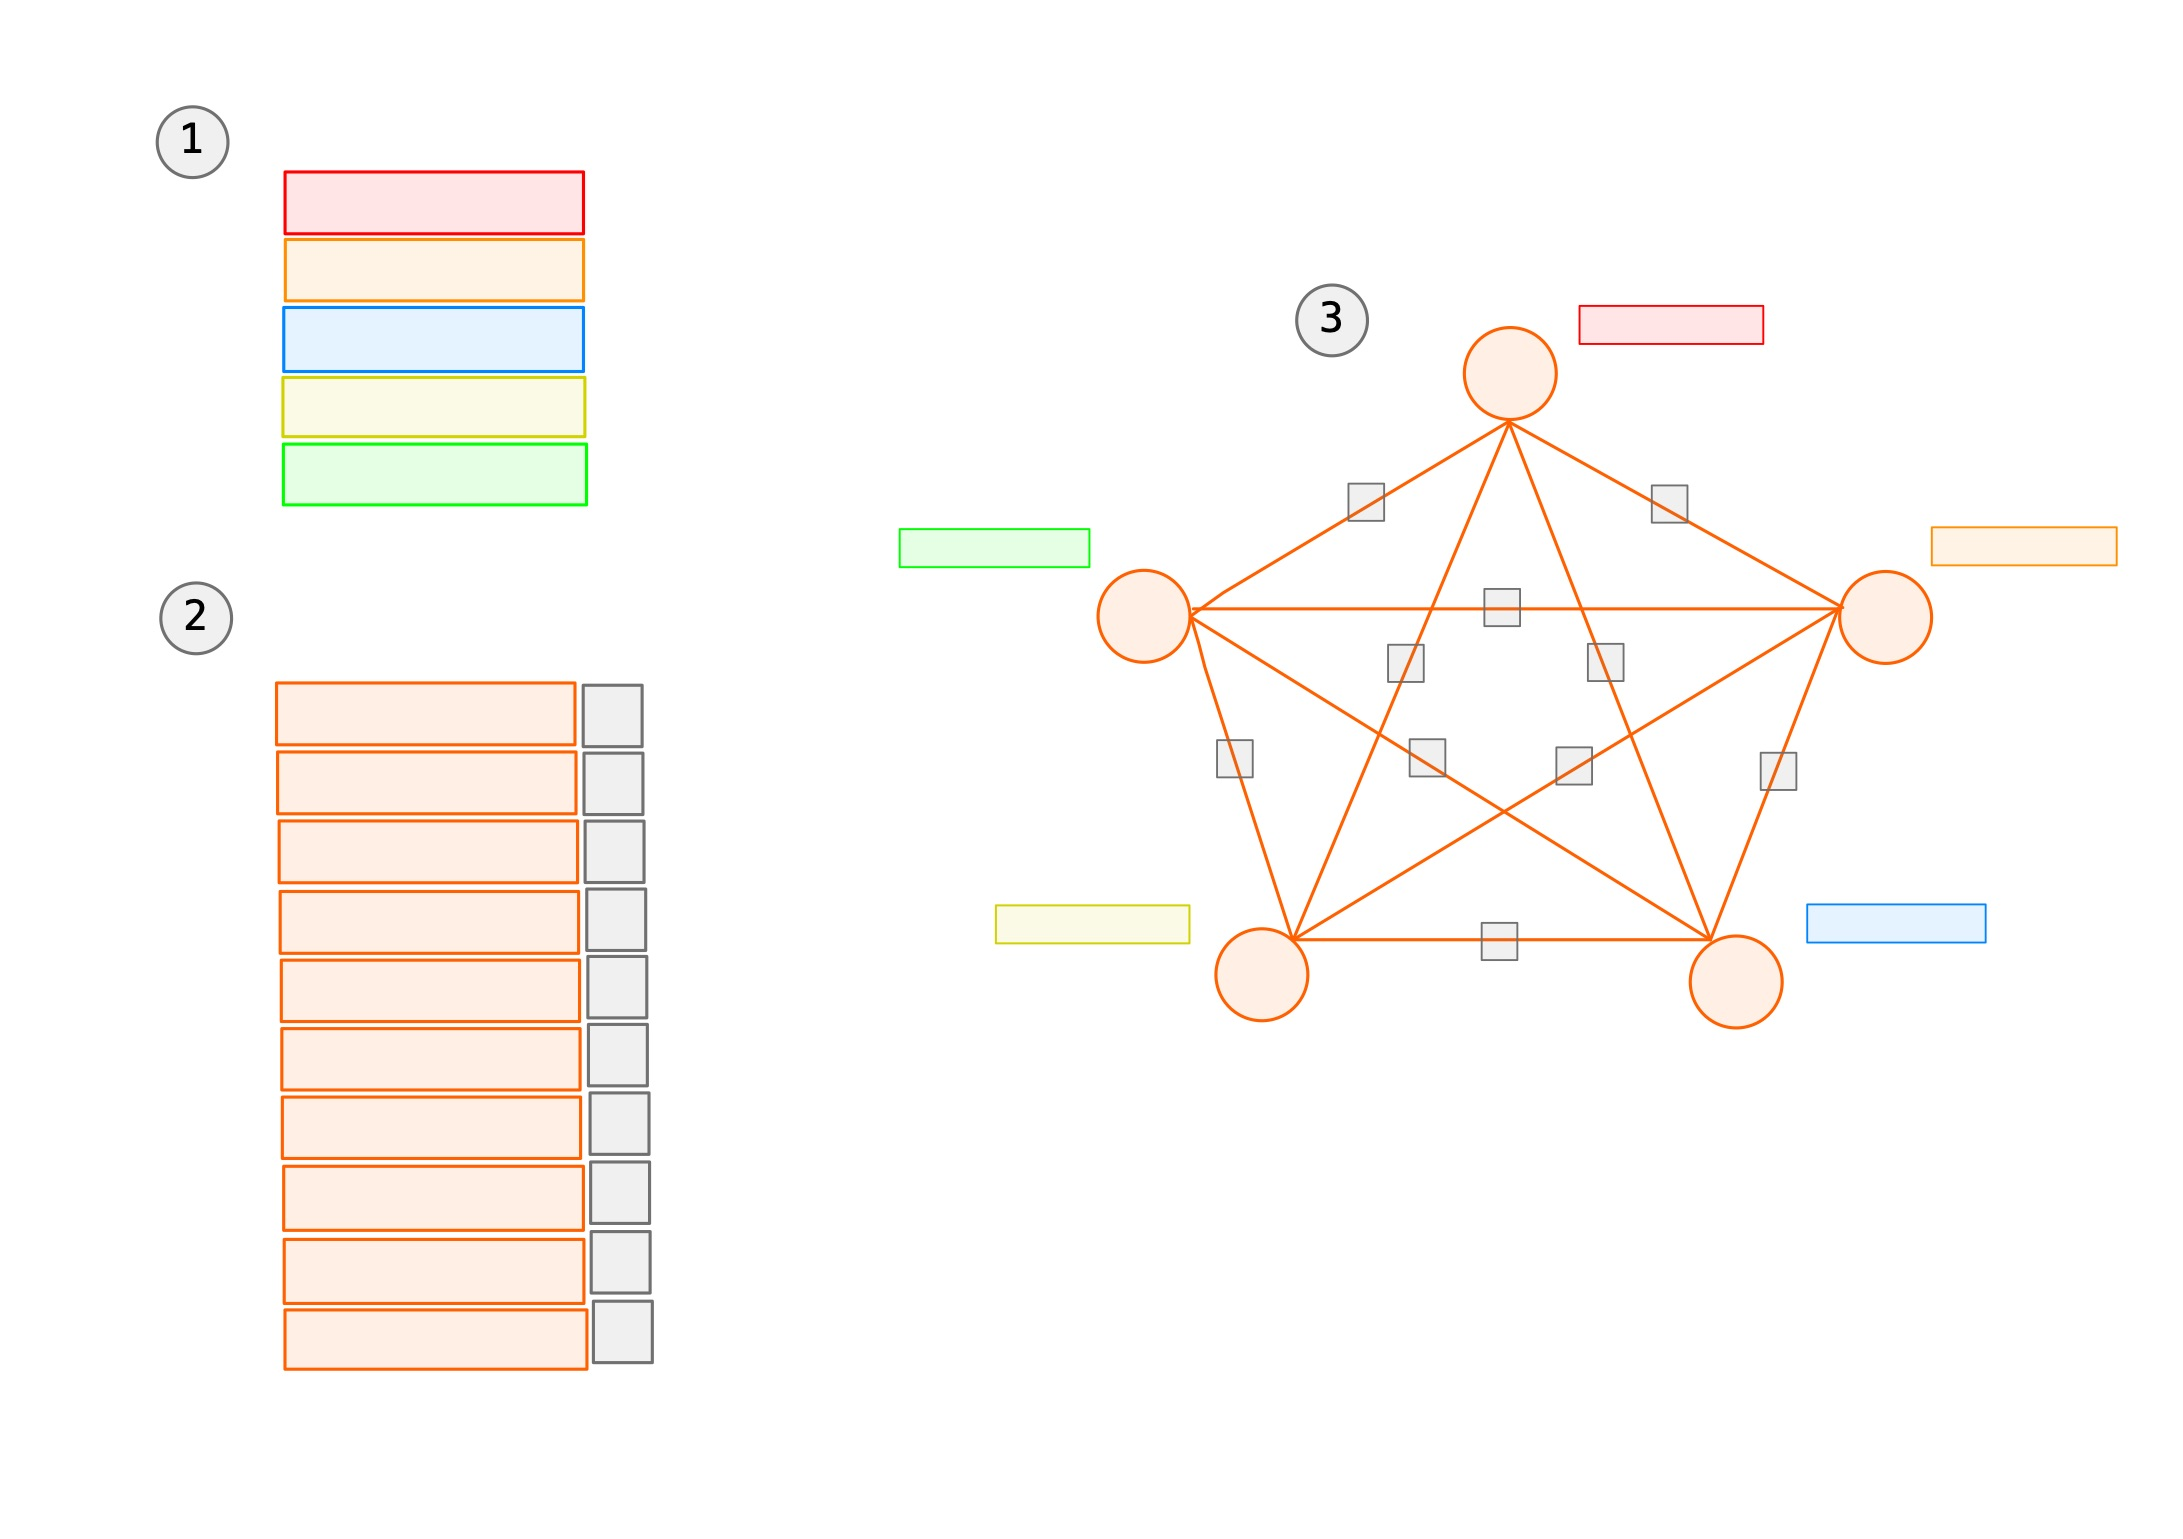
\includegraphics[width=\textwidth]{gcn-data.jpg}
  \caption{Overview of GCN dataset creation procedure. \textbf{(1)} an
    example of the main dataset with 5 hits. \textbf{(2)} the
    corresponding modified MLP dataset created. Although the dataset
    will contain $n^{2}-n = 25$ rows, only the unique rows (10 in this
    example) are shown in the illustration for simplicity.
    \textbf{(3)} The graph representation is created where rows of (1)
    become the node embeddings and the label column of (2) become the
    edge weights.}
  \label{fig:gcn-data}
\end{figure}

A modified MLP dataset (see \ref{sec:mlp-data-prep}) with a shape of
\texttt{$(n^{2}-n, 5)$} is created such that each hit is paired with
all other hits except itself. The label column from this dataset is
then used as the edge weights of the graph. Edges between event nodes
from the same event thus are assigned a weight of 1 and all other
edges are assigned a weight of 0.

Since the main dataset and the pattern matrix dataset are highly
skewed, naturally the GCN dataset is also skewed with majority of the
nodes being noise. Similar strategy as used in the creation of the
pattern matrix training set (see \ref{sec:mlp-data-prep}) is
used. The training set is a graph with 1000 nodes equally distributed
amongst the classes.

The skewed nature of the data is maintained in the testing set. The
model is evaluated with 3 test sets each with varying levels of
examples of event nodes. In practise, the pipeline will observe
timeslices with no to very few events thus the performance of the
model on test set 1 and 2 should be given importance.

\begin{enumerate}
\item[\textbf{TS1}.] No event nodes
\item[\textbf{TS2}.] Less than 25 event nodes
\item[\textbf{TS3}.] Less than 250 event nodes
\end{enumerate}

\section{Model Description and Evaluation}
\label{sec:gcn-model-desc-eval}

The model is expected to classify nodes of an unseen graph as event or
noise nodes. Since causally related nodes are connected with edges
carrying a high weight, the model is expected to group them together
thus resulting in a final graph with small clusters of causally
related nodes and a large clusters of noise nodes.

\begin{table}[t]
  \centering
  \begin{tabular}{rr}
    \hline
    Loss & BCELoss \\
    Optimizer & Adam with learning rate of $0.001$ \\
    Hidden Activation & ReLu \\
    Output Activation & Sigmoid \\
    \hline
  \end{tabular}
  \caption{GCN Model Parameter Summary.}
  \label{tab:gcn-model-param}
\end{table}

The parameters of the model are summarized in Table
\ref{tab:gcn-model-param}, the rational for selecting the parameters
being the same as that of the pattern matrix model (see
\ref{sec:mlp-model-desc}) since both models perform binary
classification. The difference comes from the model architecture. The
GCN model comprises of an input layer, two graph convolusional layers
and an output layer. The network is fully connected with 4 neurons in
the input layer, 16 in both graph convolusional layers and 1 neuron in
the output layer.

Evaluation metrics used for evaluating the MLP model are used to
evaluate the GCD model as well (see Section \ref{sec:mlp-model-eval})
since the GCN dataset is also highly skewed in nature.

\section{Discussion}
\label{sec[gcd-disc]}
% primitive weights
% medium
%% ROC AUC: 0.875
%% PR AUC: 0.064
%%               precision    recall  f1-score   support

%%          0.0       1.00      0.58      0.73       982
%%          1.0       0.04      1.00      0.08        18

%%     accuracy                           0.58      1000
%%    macro avg       0.52      0.79      0.40      1000
%% weighted avg       0.98      0.58      0.72      1000

%% F1 score: 0.079
%% F2f score: 0.178

% high
%% ROC AUC: 0.812
%% PR AUC: 0.358
%%               precision    recall  f1-score   support

%%          0.0       1.00      0.58      0.73       782
%%          1.0       0.40      1.00      0.57       218

%%     accuracy                           0.67      1000
%%    macro avg       0.70      0.79      0.65      1000
%% weighted avg       0.87      0.67      0.70      1000

%% F1 score: 0.571
%% F2f score: 0.769

% adv weights
% medium
%% ROC AUC: 1.0
%% PR AUC: 1.0
%%               precision    recall  f1-score   support

%%          0.0       1.00      1.00      1.00      1019
%%          1.0       1.00      1.00      1.00        10

%%     accuracy                           1.00      1029
%%    macro avg       1.00      1.00      1.00      1029
%% weighted avg       1.00      1.00      1.00      1029

%% F1 score: 1.000
%% F2f score: 1.000

% high
%% ROC AUC: 1.0
%% PR AUC: 1.0
%%               precision    recall  f1-score   support

%%          0.0       1.00      1.00      1.00      1043
%%          1.0       1.00      1.00      1.00       238

%%     accuracy                           1.00      1281
%%    macro avg       1.00      1.00      1.00      1281
%% weighted avg       1.00      1.00      1.00      1281

%% F1 score: 1.000
%% F2f score: 1.000
% ---------------------------------------------------------------------------
% ----------------------- end of thesis sub-document ------------------------
% ---------------------------------------------------------------------------
